\begin{exercise}[
    tags    = {frecuencia, fotón, radiación, energía, longitud de onda, constante de Plank},
    topics  = {química, física, cuántica, Plank},
    source  = {FQ 1B OXF 2015, p103, e32},
  ]
  Calcula la energía del fotón correspondiente a una radiación de frecuencia \SI{6e14}{s^{-1}}. Determina la longitud de onda de esa radiación.
\end{exercise}

\begin{solution}
  \SI{3.98e-19}{\joule}; \SI{500}{\nano\meter}
\end{solution}



\begin{exercise}[
    tags    = {números cuánticos, electrones, átomo},
    topics  = {química, cuántica, modelos atómicos},
    source  = {EBAU-Q 2013, extraordinaria fase general},
  ]
  Indique el valor, o valores, posibles para cada uno de los números cuánticos que faltan. Justifique la respuesta.
  \begin{enumerate}
    \item \( n = 3 \), \( l = ? \), \( m = 2 \)
    \item \( n = ? \), \( l = 2 \), \( m = 1 \)
    \item \( n = 4 \), \( l = 2 \), \( m = ? \)
    \item \( n = ? \), \( l = 0 \), \( m = ? \)
  \end{enumerate}
\end{exercise}

\begin{solution}
  \begin{enumerate}
    \item Para \( n = 3 \), \( l \) puede tomar los valores 0, 1 y 2. Puesto que \( m = 2 \) y este número varía entre \(–l\) y \(+l\) pasando por cero, necesariamente \( l = 2 \).
    \item Dado que los valores de \(l\) van desde 0 a \( n-1 \), si \( l = 2 \), n debe tener un valor de 3 o superior.
    \item Los valores de \(m\) varían desde \(–l\) a \(+l\) pasando por cero. Luego los valores posibles de \(m\) son \(-2\), \(-1\), 0, \(+1\), \(+2\).
    \item Para \( l = 0 \), necesariamente \( m = 0 \). Puesto que los valores de \(l\) varían desde 0 a \( n – 1 \), \(n\) debe tener un valor igual o superior a 1.
  \end{enumerate}
\end{solution}



\begin{exercise}[
    tags    = {configuración electrónica, electrones, átomo, ión},
    topics  = {química, cuántica, modelos atómicos},
    source  = {EBAU-Q 2013, ordinaria específica},
  ]
  Escriba las configuraciones electrónicas de los iones \ch{X^{2+}} \( (Z = 20) \) e  \ch{Y^{2-}} \( (Z = 34) \) e indique el grupo y período de la tabla periódica al que pertenecen los elementos de los que derivan estos iones.
\end{exercise}

\begin{solution}
  \begin{itemize}
    \item \ch{X^{2+}} \( (Z = 20) \):  \( 1s^2,2s^22p^6,3s^23p^6 \). Grupo 2, período 4.
    \item \ch{Y^{2-}} \( (Z = 34) \):  \( 1s^2,2s^22p^6,3s^23p^63d^{10},4s^24p^6 \). Grupo 16, período 4.
  \end{itemize}
\end{solution}




\begin{exercise}[
    tags    = {clorhídrico, CO2, HCl, CaCO3, disolución, porcentaje en masa, densidad},
    topics  = {química, reaccion, estequiometría, disoluciones},
    source  = {FQ 1B ANA 2015, p117, e38},
  ]
  En el laboratorio se puede obtener \ch{CO2} haciendo reaccionar \ch{CaCO3} con \ch{HCl}; en la reacción también se produce \ch{CaCl2}. Se quieren obtener \SI{5}{\liter} de dióxido de carbono, medidos a \SI{25}{\celsius} y \SI{745}{\mmHg}. Suponiendo que hay suficiente carbonato de calcio, calcula el volumen mínimo de ácido clorhídrico al 32\% en masa y densidad \SI{1,16}{\gram\per\liter} que será necesario utilizar.
\end{exercise}

\begin{solution}
  \SI{39,2}{\milli\liter} de \ch{HCl}.
\end{solution}



\begin{exercise}[
    tags    = {entalpía, entalpia de reacción, calor, entropía, energía de Gibbs},
    topics  = {química, termoquímica, termodinámica, espontaneidad},
    source  = {FQ 1B ANA 2016, p166, e32},
  ]
  Utilizando los valores que aparecen en la tabla, todos ellos obtenidos a la temperatura de \SI{25}{\celsius}, para la siguiente reacción de obtención del fosgeno:
  \[ \ch{CO (g) + Cl2 (g) -> COCl2 (g)} \]

  \begin{enumerate}
    \item Indica si será o no espontánea y si este hecho depende de la temperatura.
    \item Calcula la energía transferida al formarse \SI{5}{\gram} de fosgeno e indica, justificando tu respuesta, si se desprende o se absorbe la energía en el proceso.
  \end{enumerate}

  \begin{gexdatos}
    \begin{tabular}{ccc}
      Sust. & \( \Delta H^0_f \) (\si{\kilo\joule\per\mole}) & \( S^0 \) (\si{\joule\per\kelvin\per\mole}) \\
      \toprule
      \ch{CO (g)} & \( -110,4 \) & \( 197,7 \) \\
      \ch{Cl2 (g)} & \( 0,0 \) & \( 223,1 \) \\
      \ch{COCl2 (g)} & \( -222,8 \) & \( 288,8 \) \\
      \bottomrule
    \end{tabular}
  \end{gexdatos}
\end{exercise}

\begin{solution}
  \begin{enumerate}
    \item La reacción es espontánea a \SI{289}{\kelvin}.
    \item \( \Delta H_r = \SI{-5.68}{\kilo\joule} \).
  \end{enumerate}
\end{solution}


\begin{exercise}[
    tags    = {tiro oblicuo, MRU, MRUA, caída},
    topics  = {física, cinemática, composición de movimientos},
    source  = {FQ 1B SM 2015, p248, e50},
  ]
  Un gran peñasco descansa en la cima de un barranco de \SI{80}{\meter} de altura, por encima de un pueblo. Se encuentra en una posición al que si rodase hacia abajo saldría despedido con una velocidad de \SI{20}{\meter\per\second} en un ángulo de \ang{30} con respecto de la vertical.

  Las casas del pueblo se encuentran a \SI{50}{\meter} de la base del barranco. ¿Tiene la población motivos para sentirse insegura? Si el peñasco cayera, ¿cuánto tiempo estaría en el aire? ¿Cuál sería el módulo de su velocidad al impactar en el suelo?
\end{exercise}

\begin{solution}
  \SI{2.6}{\second}; \SI{44}{\meter\per\second}
\end{solution}



\begin{exercise}[
    tags    = {dinámica, poleas, rozamiento, bloques, cuerpo libre},
    topics  = {física, dinámica, leyes de newton},
    source  = {FQ 1B OXF 2015, p331, e19},
  ]
  En el sistema dibujado, las masas valen \( m_a = \SI{15}{\kilo\gram} \),
  \( m_b = \SI{5}{\kilo\gram} \) y \( m_c = \SI{3}{\kilo\gram} \), y el coeficiente de rozamiento \(\mu\) entre \( m_b \)  y \( m_c \), es de 0,3. Si los demás rozamientos son despreciables (así como las masas de las poleas y la cuerda), halla la aceleración del sistema y las tensiones de las cuerdas.
  \begin{figure}[h]
    \centering
    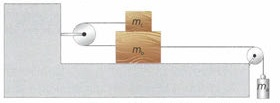
\includegraphics{FQ_1B_OXF_2015_p331e19}
  \end{figure}
\end{exercise}

\begin{solution}
  \SI{5,62}{\meter\per\square\second}; \( T = \SI{62,7}{\newton} \); \( T' = \SI{25,7}{\newton} \)
\end{solution}




\begin{exercise}[
    tags    = {energía cinética, energía potencial, trabajo, energía mecánica},
    topics  = {física, energía, trabajo},
    source  = {propio},
  ]
  Un camión con una masa de \SI{20}{t} desciende por la autopista del Huerna a \SI{90}{\kilo\meter\per\hour} cuando, súbitamente, sus frenos dejan de funcionar y comienza a descender sin control. Para evitar un accidente, el conductor decide sabiamente dirigirse a la siguiente rampa de frenado, que se encuentra casualmente a \SI{500}{\meter}. La pendiente media de la autopista es del 6\% (\ang{4} aprox.) y podemos considerar que el rozamiento del asfalto es despreciable. La rampa de frenado, por el contrario, se encuentra perfectamente horizontal, mide \SI{150}{\meter} y su coeficiente de rozamiento es de 0,6. ¿Será suficiente para detener al camión, o debemos esperar un trágico desenlace?
\end{exercise}

\begin{solution}
  El camión frena en \SI{200}{\meter}, luego sí que es suficiente. ¡Hemos salvado el día!
\end{solution}
